%-----<<< INTRO >>>-----
\chapter{Introduction}
\label{ch:intro}

Biomimetic \textit{flapping-wing micro-aerial vehicles} (FWMAV) have been the focus of much recent research due to their potential for both civilian and military applications. Because of heir insect-like size and relative simplicity in comparison with more traditional unmanned aerial systems (such as quadrotors or fixedwing airplanes), they can be made relatively cheaply and be a part of personal equipment of soldiers, first responders, law enforcement members etc. Probably the most well-known is their application in military reconnaissance -- a soldier launches the drone in the air to get a better view of the battlefield, and to spot enemies and obstacles. Small pocket-size drones are already being tested for military use \cite{proxdynamics}. Similarly, insect-like robots can be used for law enforcement and surveillance -- helping SWAT teams locate suspects, or monitor crowds. Ground robots capable of stealthy surveillance are already available \cite{throwbot}. 

Firefighters use drones to monitor fire from above \cite{firedrone}, but an insect-like drone can fly inside a burning building and help access the fire damage without exposing fire crew to danger. First responders would benefit from miniature drones that map dangerous environments before humans step in, and that measure radiation and toxic levels in contaminated areas (if equipped with proper sensors) after a fire or an environmental disaster. One application unique for miniature flapping-wing robots is artificial pollination -- in the catastrophic event that there is not enough bees available, robotic pollinators can take over and help farmers where needed \cite{robopollination}. Yet another, perhaps more exotic use is planetary exploration as suggested by \cite{Brooks1989}.

In either possible application area, adaptive, fault-tolerant, control and autonomous operation is paramount. One way to achieve the desired level of autonomy is with a \textit{Multi Agent System} (MAS) -- where different agents inside of the robot's controller are responsible for specific tasks. For example, one agent is responsible for adapting the flight trajectory, while a second agent is responsible for monitoring the "health" of the robot, and a third agent can help during a fault recovery. This way even a very complex system can be split into simpler tasks. %More information about MAS can be found in Section~\ref{sec:MAS}.
\textit{Subsumption architecture}, another concept well known in robotics described in Section~\ref{sec:subsumption_arch}, is used for prioritization over different goals, which gives the robot the desired autonomy. The concept of MAS combined with the \textit{subsumption architecture} is general enough so it can be used on various robots for different applications. In our research we use evolution algorithms, which can quickly evolve the robotic control system and tune it for a particular application.

% figure: application uses
\begin{figure}
\centering
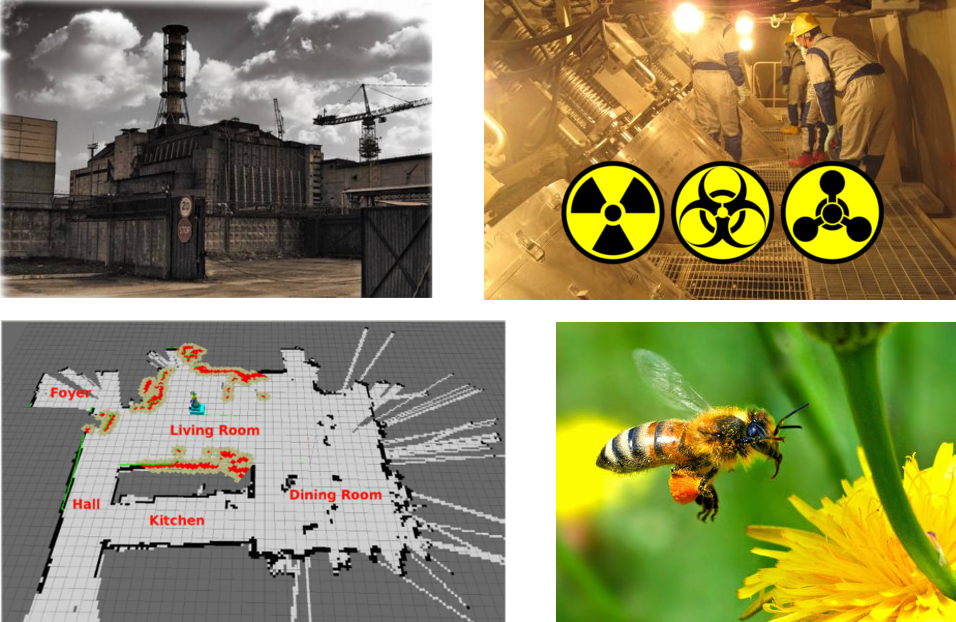
\includegraphics[width=0.8\textwidth]{Files/Figures/applications.png}
\caption[Application examples]{An example of applications of flapping-wing robots. Top left: Detecting toxic materials; Top right: Measuring radiation levels in contaminated areas; Bottom left: Mapping of dangerous environment; Bottom right: Artificial pollination}
\label{fig:application}
\end{figure}


\section{Problem Statement}
\label{sec:application}
In the aforementioned examples, the existing drones are remotely controlled by a human pilot. They have some sense of autonomy (i.e. a "hold" function that keeps the drone hovering on a spot while the operator for example pans the on-board camera), but are not able to perform fully autonomous missions. Nonetheless, greater autonomy is not always well-received by the public (for example see \cite{dailymail}), so it is important to keep the related ethical questions in mind \cite{uavethics} \cite{morallandscape}.

FWMAVs, unlike their counterparts with rotating blades and fixed wings, have the potential to be truly insect-size. The reason is that the conventional technologies used for macroscale aircrafts do not scale well, because the decreased size brings an increased dominance of surface forces, causing revolute joints or sliding sliding surfaces (for example propellers shafts and motor bearings) inefficient or even infeasible \cite{Buck2013}. In addition, the lift-to-drag ratio for fixed aerofoils decreases at small scales because of the greater effect of viscous forces relative to lift-generating inertial forces at low Reynolds numbers \cite{Fuller2014}.

A FWMAV qualifies as a \textit{Cyber Physical System} (CPS). A CPS is a system where a controlled physical process and information processing is tightly coupled. Working with CPS introduces unique challenges, which is described in Section~\ref{sec:cps}. This work describes a MAS for adaptive control of a FWMAV. The vehicle employed in this research is
similar to a minimally-actuated FWMAV introduced by Wood~\cite{Wood2008}, \cite{robobees} with core control laws introduced and subsequently refined by Doman et al. \cite{afrl1}, \cite{afrl2}. Our vehicle \cite{Perseghetti}, \cite{Boddhu}, \cite{Botha} operates similarly to the minimally actuated vehicles considered by Wood and Doman et al. in that all propulsion and control are provided by two wings, each of which possesses a single active and a single passive degree of freedom. As previously mentioned \cite{afrl1}, the two wing configuration allows full 6 DoF control and is mimicking a bee or a fly.

Previous work employed variants of the controllers discussed in \cite{afrl1}, \cite{afrl2} augmented with adaptive wing beat oscillators \cite{gallagher}, \cite{Gallagher2012a}, \cite{Gallagher3} that provided adaptation at the inner-most layer of vehicle control (wing flapping patterns). The goal of that work was to provide adaptation not by changing control laws that related desired forces and torques to stereotyped wing motions, but rather, to change the wing stereotyped motions to adapt generated forces to the needs of control laws designed for undamaged wings. In other words, the salient adaptation was that damaged wings learned to move in ways that mimicked the force and torque generation of undamaged wings. As a result the higher level controllers would not be able to distinguish between normal operation and damaged wings.

In contrast to that work, this dissertation describes a design for a MAS where control laws are directly adapted at a higher level of abstraction in the control law hierarchy. In this system, agents are responsible for collecting and estimating vehicle pose, recording waypoint locations for trajectory following, generating inputs needed by the split-cycle oscillator, monitoring vehicle behaviour and, when necessary, conducting diagnostics and adapting the control rule base. In this case the higher level control system monitors (directly or indirectly) the wing performance and adapts if necessary, while the inner-most layer of control is fixed. The initial set of control laws is designed using a combination of extrinsic and intrinsic evolution \cite{Tyrrell}. The ultimate vision is that both forms of adaptation co-exist in the vehicle so that the benefits of each approach are equally available. 



\section{Research Objectives}
\label{sec:researchObjectives}

The former approach \cite{Perseghetti}, \cite{Boddhu}, \cite{Botha} focused on lower level control, and didn't provide a complete solution. The later approach, described in this dissertation, utilizing a MAS, provides a complete high-level control as well as autonomy to the vehicle. In combination with evolution inspired techniques, the control system is able to adapt to different vehicles and to different conditions (for example damaged wings). The main contribution of our research is that it proves the viability of a MAS for a FWMAV by demonstrating the autonomous waypoint following, and the concept of likelihood based fault detection procedure. The major outcomes of this research are:

\begin{enumerate}
\item understanding the viability of a MAS for control of flapping wing vehicles
\item developing a multi-agent control system allowing the vehicle to follow trajectory in experimental settings
\item developing fault detection and fault recovery mechanisms based on a combination of extrinsic and intrinsic evolution
\item developing high degree of autonomy of the vehicle, including trajectory following and fault recovery procedures \end{enumerate}

This research is supported in part by the National Science Foundation under Grant Numbers CNS-1239196, CNS-1239171, and CNS-1239229.
